\subsection{Einleitung}
\begin{frame}{Nichtrealistische Computergraphik}
  \begin{columns}
    \column{.3\textwidth}
	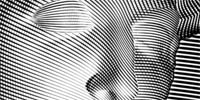
\includegraphics[width=0.9\textwidth]{../images/npr_schraffur.jpg}
	\column{.7\textwidth}
	  \begin{itemize}
	    \item non-photorealistic rendering (NPR)
% nichtrealistische computergraphik ist ein teilgebiet der computergraphik mit
% dem ziel eine grosse vielfalt an ausdrucksstarken malstilen für digitale kunst
% zur verfügung zu stellen.
% Das klingt zunächst etwas gegensätzlich, da man im Bereich der traditionellen
% Computergraphik mit hohem Aufwand versucht, möglichst photorealistische Bilder
% zu erzeugen. Aber es gibt einige Gebiete,
% zum Beispiel Cartoons, die gerade davon leben, dass die dargestellten Figuren
% nicht realistisch wirken.
%
		\item  Entstehungsgeschichte der NPR
% Erste Filme wurden bereits in den 50 Jahren gemacht, welche allerdings darauf
% beruhten ein Nagelbrett zu fotografieren und diese Fotos zu einer Animation zu
% verbinden. Mit der zunehmenden Einführung von Computern wurde nach und nach
% 	auch versucht, technische Zeichnungen am Computer anzufertigen. Der Begriff des
% 	NPR wurde aber erst in den 90er Jahren des vergangenen Jahrhunderts geprägt.
% 	Die automatische Erzeugung von Skizzen und Modellen hilft viel Arbeit zu sparen
% 	und Änderungen schnell möglich zu machen.

	    \item Wozu wird es eingesetzt?
	% Um comichafte Darstellungen zu erreichen, kann man in einem Animationsprogramm
	% Toonshader einsetzen, was eines der besten Beispiele für nichtrealistische
	% Computergraphik darstellt. Aber auch in 2D-Programmen kennt man Algorithmen
	% des NPR, beispielsweise in einem Zeichenprogramm wenn man Kohleschraffurfilter
	% oder Aquarellfilter anwendet. Darauf werden wir nachher noch genauer eingehen.
      \end{itemize}
   \end{columns}
\end{frame}

\begin{frame}{Beispiele}
  \begin{columns}
    \column{.6\textwidth}
	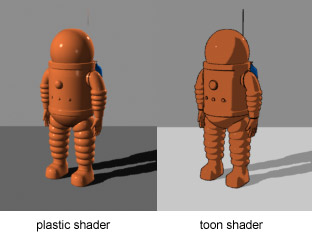
\includegraphics[width=\textwidth]{../images/Toon-shader.jpg}
	\column{.4\textwidth}
	Toon-Shader mit Borderdetection\\
	Quelle: Wikipedia
  \end{columns}
\end{frame}

\begin{frame}{Transformationsformen}
	\begin{itemize}
	  \item 2D-Bild $\rightarrow$ 2D-Bild (Kohleschraffur, Wasserfarben, \ldots)
	  \item 3D-Modell $\rightarrow$ 2D-Bild (Bäume)
	  \item 3D-Modell $\rightarrow$ 3D-Modell (veränderte Texturen, Modell wirkt
	  "`zweidimensionaler")
	\end{itemize}
\end{frame}